\section{Volume exploration}
\label{sect:volume-exploration}

Figure~\ref{fig:tf-design-example} illustrates our TF design interface: a 2D scatter plot where each point represents a volume FOI. The coordinates of the points are determined by the FastMap projection. Each point corresponds to a pivot (the centroid of a cluster), with its radius proportional to the number of voxels it represents, normalized logarithmically. It is important to highlight that each pivot results from a two-level clustering process, generated by the combination of SSS and DBSCAN.

\begin{figure}[htb!]
    \centering
    \subfloat[Initial transfer function definition.\label{subfig:tf-design-example-generated}]{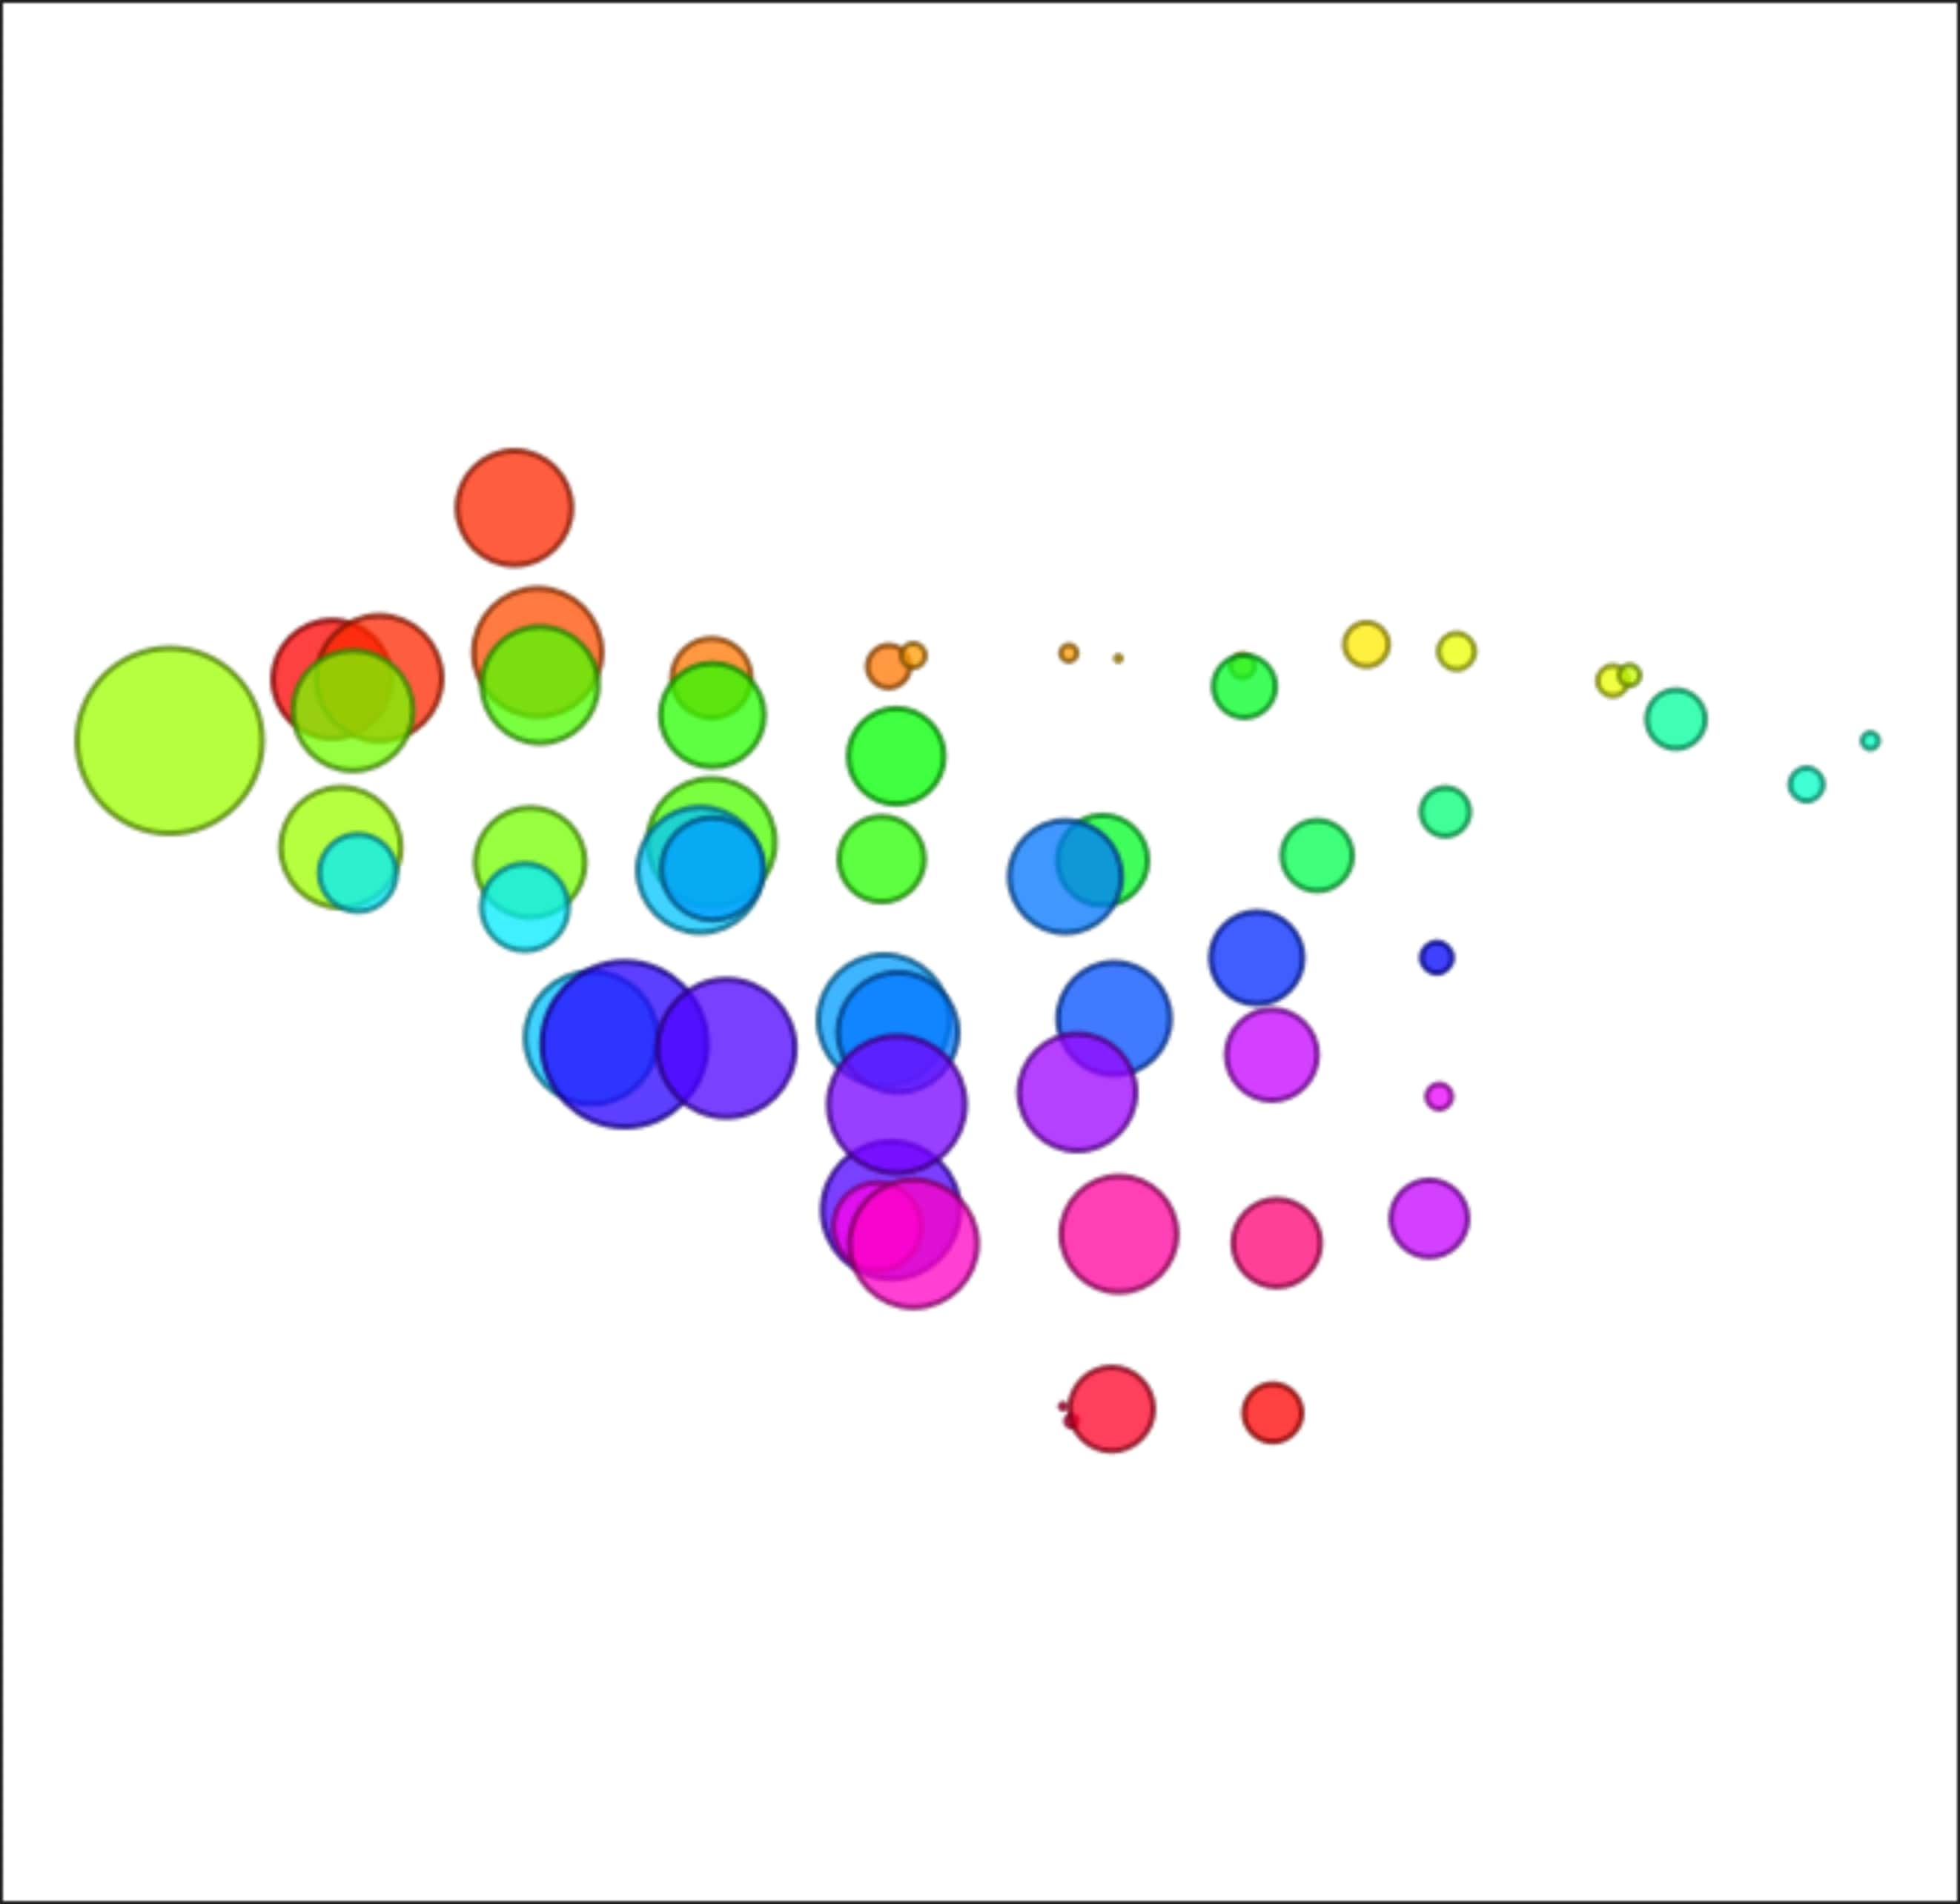
\includegraphics[width=0.47\columnwidth]{figs/tf-design-interface-a.jpg}}
    \hfill
    \subfloat[Fine-tuned transfer function definition after user adjustment over identified volume features of interest.\label{subfig:tf-design-example-user}]{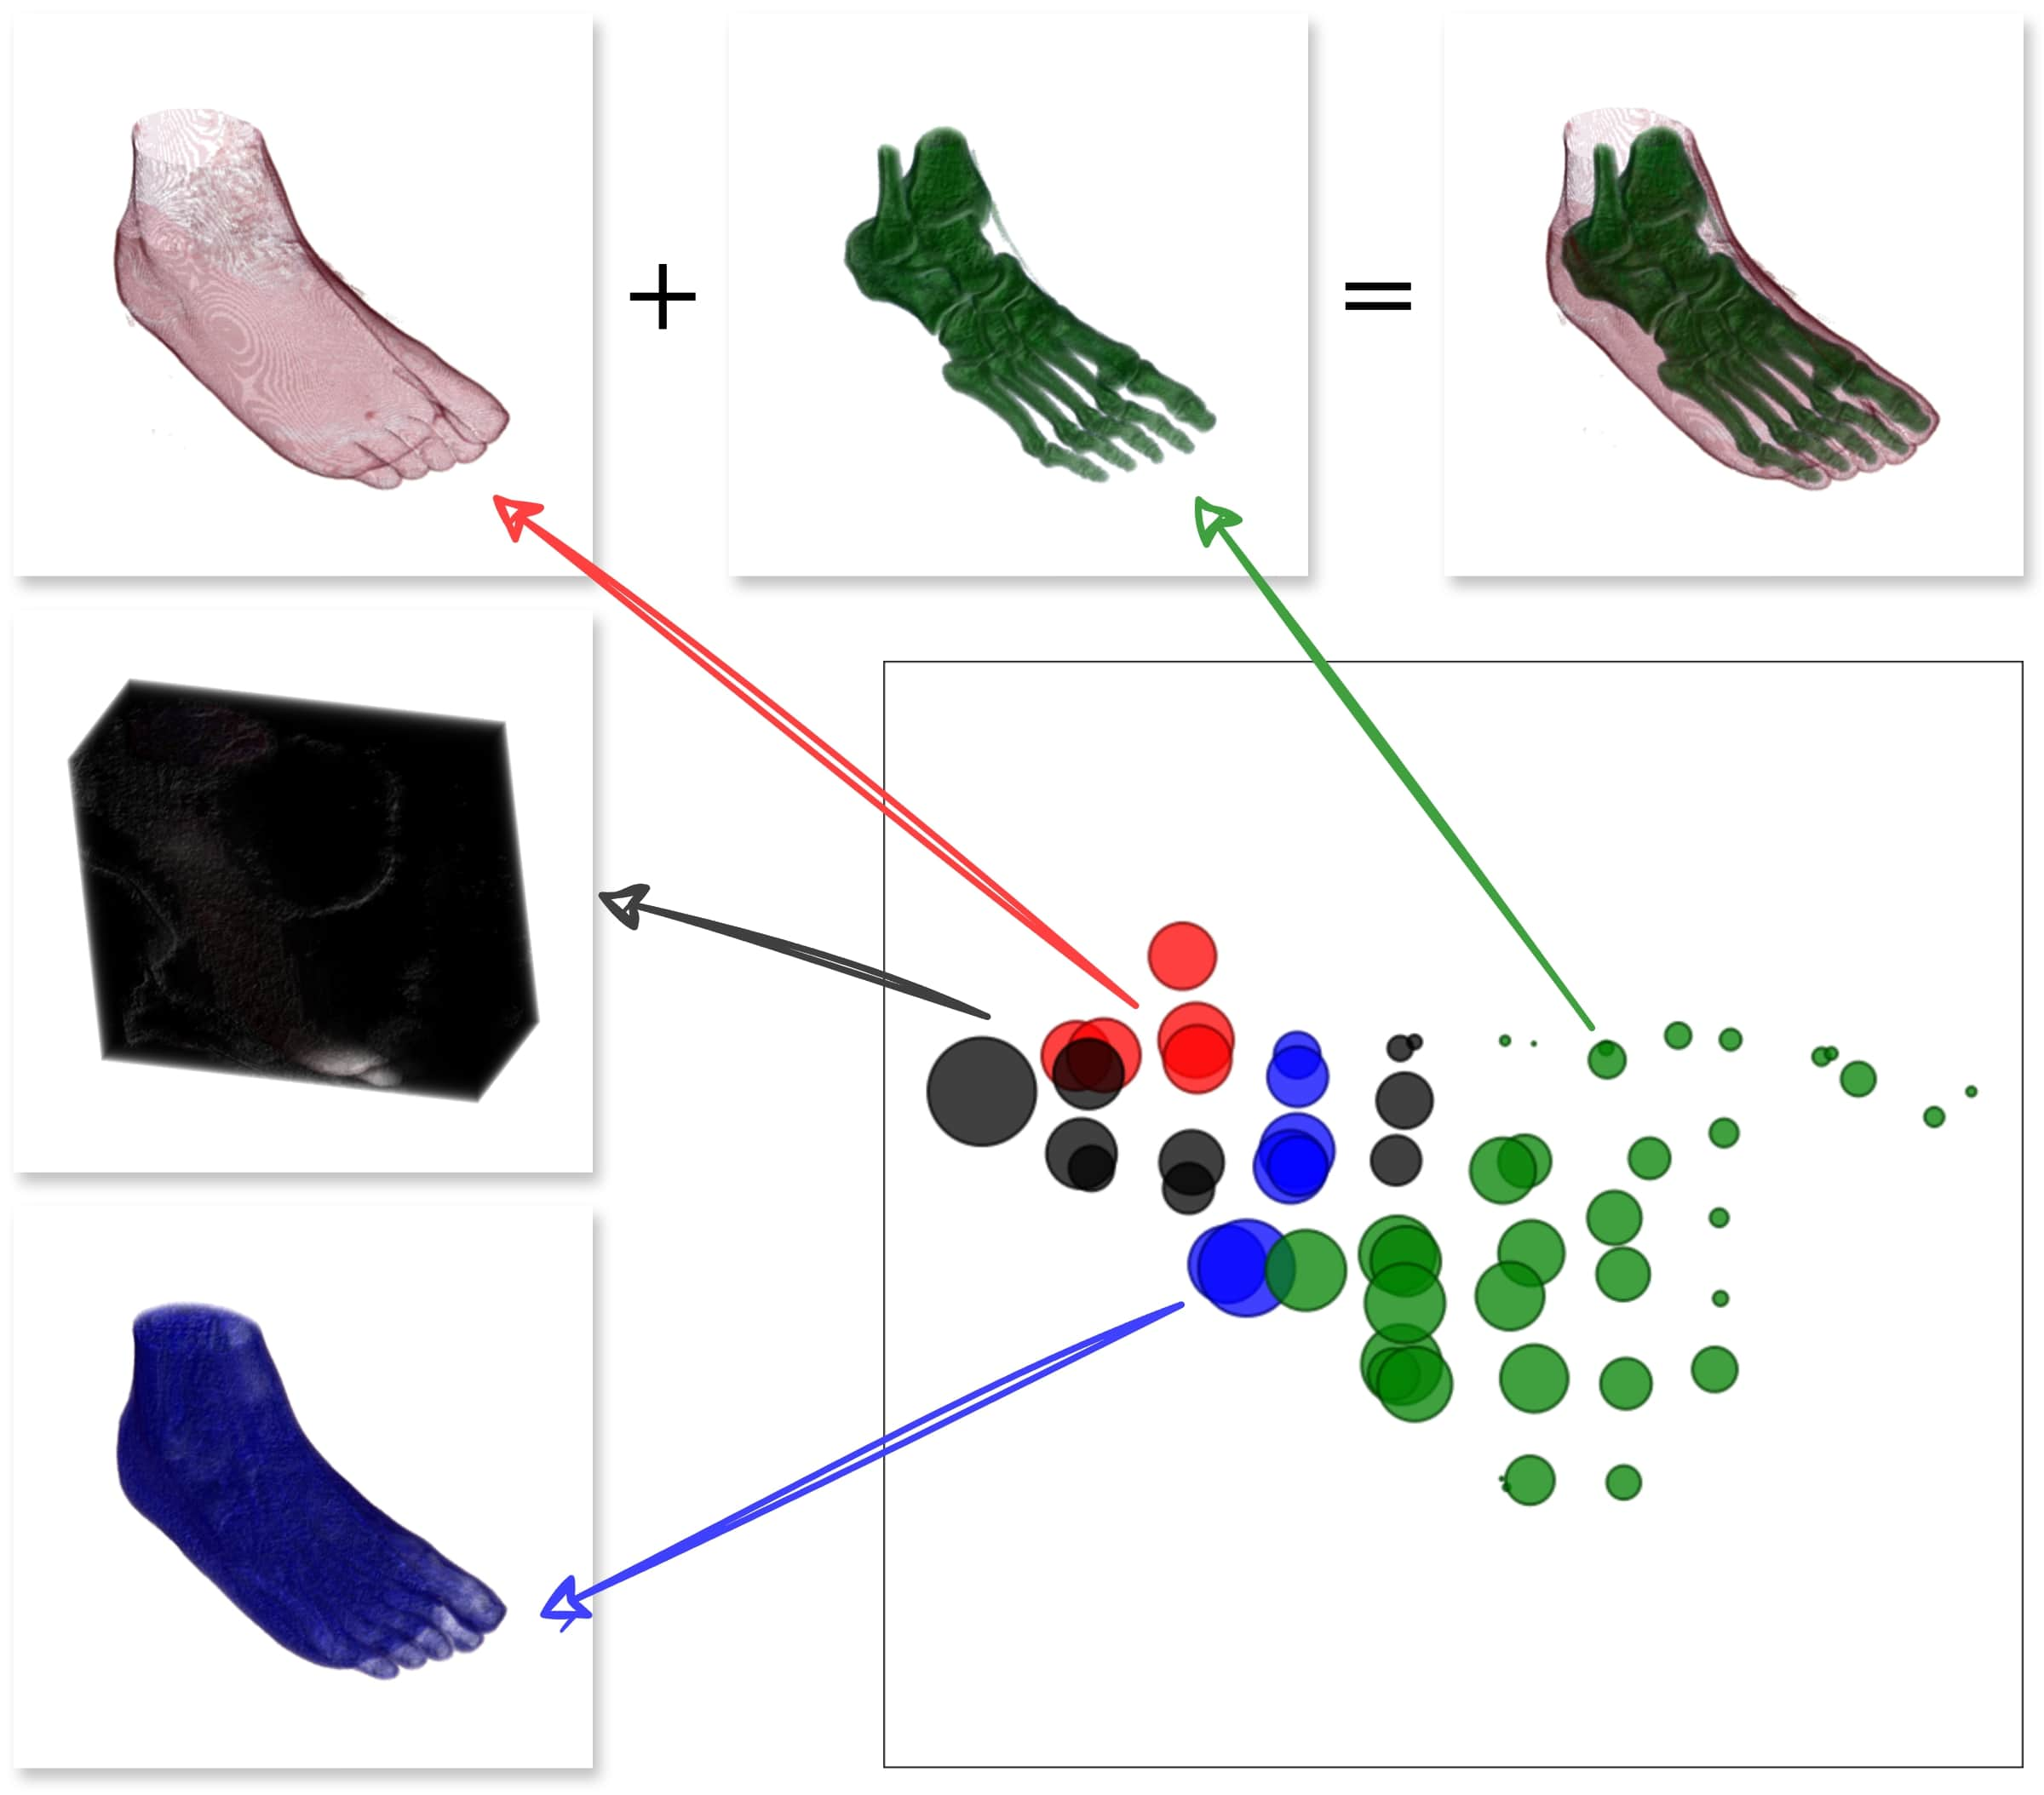
\includegraphics[width=0.47\columnwidth]{figs/tf-design-interface-b.jpg}}
    \caption{Transfer function design interface and interactive volume exploration of a right male foot dataset.}
    \label{fig:tf-design-example}
\end{figure}

Our method generates an initial TF definition using a predefined opacity and a rainbow color scale, assigning a unique color to each cluster.

Users adjust the TF definition following the WYSIWYG principle: the pivot’s color and opacity directly map to their associated voxels according to clustering. Both selected and unselected elements are fully customizable.

Volume exploration is performed through pivot selection. The system dynamically increases the opacity of selected pivots while decreasing that of others. Users can make arbitrary selections, save them as groups, and interact with pivots, clusters, or groups as selectable entities.

Iterative selection of nearby elements facilitates detailed inspection of volume structures. FastMap and DBSCAN naturally cluster spatially similar FOIs, simplifying this process.

Our approach automates material classification by assuming each cluster or pivot corresponds to a relevant item. If users are unsatisfied, they may select or deselect elements or adjust the following parameters:

\begin{itemize}
    \item input data attributes,
    \item DBSCAN parameters $\varepsilon$ and $minPts$,
    \item SSS distance factor $\alpha$.
\end{itemize}
